\documentclass[11pt]{article}
\usepackage[margin=1.1in]{geometry}
\usepackage[sc]{mathpazo}
\linespread{1.06}
\usepackage{amsmath,amssymb,amsthm,mathtools}
\usepackage{microtype}
\usepackage{enumitem,booktabs,array}
\usepackage{tikz}
\usetikzlibrary{arrows.meta,positioning,calc,fit}
\usepackage{xcolor}
\usepackage[most]{tcolorbox}
\definecolor{linkblue}{RGB}{25,63,105}
\definecolor{ideabg}{RGB}{244,241,232}
\definecolor{idearule}{RGB}{150,120,60}
\usepackage[colorlinks=true,allcolors=linkblue]{hyperref}
\usepackage[nameinlink,capitalise,noabbrev]{cleveref}
\hypersetup{pdftitle={L = RL = BPL: An Expository Account},
  pdfsubject={Expository rewrite of OpenAI's manuscript Exact Derandomization of Logarithmic Space (2026)}}

\newtheorem{theorem}{Theorem}[section]
\newtheorem{lemma}[theorem]{Lemma}
\newtheorem{proposition}[theorem]{Proposition}
\newtheorem{corollary}[theorem]{Corollary}
\newtheorem{fact}[theorem]{Fact}
\theoremstyle{definition}
\newtheorem{definition}[theorem]{Definition}
\newtheorem{example}[theorem]{Example}
\theoremstyle{remark}
\newtheorem{remark}[theorem]{Remark}

\newtcolorbox{idea}[1][]{enhanced,breakable,colback=ideabg,colframe=idearule,
  boxrule=0pt,leftrule=2.5pt,arc=0pt,outer arc=0pt,left=8pt,right=8pt,top=5pt,bottom=5pt,
  fonttitle=\bfseries\small,coltitle=idearule!70!black,
  title={#1},attach title to upper={\ \ },before skip=10pt,after skip=10pt}

\newcommand{\F}{\mathbb F}
\newcommand{\E}{\mathbb E}
\newcommand{\eps}{\varepsilon}
\newcommand{\V}{\mathcal V}
\newcommand{\cE}{\mathcal E}
\newcommand{\cG}{\mathcal G}
\newcommand{\cA}{\mathcal A}
\newcommand{\cS}{\mathcal S}
\newcommand{\rs}{r_{\mathrm s}}
\newcommand{\bpi}{\bar\pi}
\DeclareMathOperator{\OPT}{OPT}
\DeclareMathOperator{\val}{val}
\DeclareMathOperator{\Hom}{Hom}
\DeclareMathOperator{\im}{im}
\DeclareMathOperator{\rank}{rank}
\DeclareMathOperator{\Span}{span}
\DeclareMathOperator{\TV}{TV}
\DeclareMathOperator{\Tr}{Tr}
\DeclareMathOperator{\Mat}{Mat}
\newcommand{\abs}[1]{\lvert #1\rvert}
\newcommand{\ip}[2]{\langle #1,#2\rangle}
\setlist{topsep=3pt,itemsep=2pt,parsep=0pt}
\allowdisplaybreaks[1]
\setlength{\emergencystretch}{2em}

\newcommand{\Lc}{\mathsf L}
\newcommand{\RL}{\mathsf{RL}}
\newcommand{\BPL}{\mathsf{BPL}}
\newcommand{\one}{\mathbf 1}


\title{\textbf{$\mathsf L=\mathsf{RL}=\mathsf{BPL}$}\\[4pt]
\large An expository account of the proof}
\author{A rewrite, for human readers, of the manuscript\\ \emph{Exact Derandomization of
Logarithmic Space: $\mathsf L=\mathsf{RL}=\mathsf{BPL}$}\\
(OpenAI, September 23, 2026)\\[6pt]
\small Prepared with Claude (Anthropic) \quad$\cdot$\quad October 7, 2026}
\date{}

\begin{document}
\maketitle

\begin{abstract}
\noindent
In September 2026 OpenAI posted a 108-page manuscript, written by an internal
model, claiming a deterministic logarithmic-space simulation of every
bounded-error randomized logarithmic-space computation that runs in polynomial
time. In fact it approximates the acceptance probability itself to any fixed
inverse-polynomial accuracy in deterministic logarithmic space. The manuscript
is complete in the sense that every step is written down, but it is very hard
to read: ideas are introduced exactly when needed and rarely motivated. This
note explains the architecture of the proof for a complexity theorist. The
first, purely algebraic, half (a ``correction and copy hierarchy'' that pushes
all acceptance probability into a reward vector in $O(\log n)$ stages) is
elementary and is presented with full proofs. The second half (estimating that
reward with $O(\log n)$ shared random bits, then enumerating them, all in
$O(\log n)$ space) is a long chain of interlocking devices; for each one this
note explains what problem it solves, states what is proved, and points to the
manuscript. Unlike the Unique Games result in the same release, this one has no
Lean formalization. \Cref{sec:reader} says what was checked here and where a
referee should concentrate.
\end{abstract}

{\small\setlength{\parskip}{0pt}\tableofcontents}
\clearpage

\section{Introduction}\label{sec:intro}

\subsection{The claims}

Machines have a read-only input, finitely many work tapes, and fresh fair coins;
space counts every work cell visited. $\RL$ and $\BPL$ are the languages decided
by polynomial-time randomized $O(\log n)$-space machines with one-sided error
(acceptance probability $0$ versus $\ge1/2$) and two-sided error ($\le1/3$ versus
$\ge2/3$). Write $B=\Theta(\log(n+2))$ throughout.

\begin{theorem}[Theorem~1.1 of \cite{OpenAI-BPL}]\label{thm:main}
$\Lc=\RL=\BPL$.
\end{theorem}

The proof does not use the gap. It approximates the acceptance probability.

\begin{theorem}[Theorems~1.2 and 12.1 of \cite{OpenAI-BPL}]\label{thm:approx}
Let $\mathcal M$ be a randomized machine running in polynomial time and
$O(\log n)$ space, with acceptance probability $p_{\mathcal M}(x)$. For every fixed
$d$ there is a deterministic $O(\log n)$-space, polynomial-time transducer that
outputs a dyadic $z_x$ with $\abs{z_x-p_{\mathcal M}(x)}\le(n+2)^{-d}$. With the
accuracy given in unary as $1^q$, one algorithm achieves error $2^{-q}$ in space
$O(\log n+q)$ and time $n^{O(1)}2^{O(q)}$.
\end{theorem}

Consequences proved in the manuscript include $\mathsf{PromiseBPL}=\mathsf{PromiseL}$,
deterministic log-space construction of an accepting computation whenever the
acceptance probability is at least inverse-polynomial (\cref{sec:consequences}),
and an effective compiler that turns a randomized machine with stated resource
bounds into a deterministic one with explicit bounds.

\subsection{Context}

The best previous general results were Nisan's $O(\log^2n)$-space pseudorandom
generator~\cite{Nisan92}, his simultaneous polynomial-time,
$O(\log^2n)$-space simulation~\cite{Nisan94}, the Saks--Zhou
$O(\log^{3/2}n)$-space simulation~\cite{SaksZhou}, and Hoza's improvement to
$O(\log^{3/2}n/\sqrt{\log\log n})$~\cite{Hoza21}. Reingold's theorem~\cite{Reingold}
settled undirected connectivity, and Cheng and Hoza~\cite{ChengHoza} showed that
log-space hitting sets for read-once branching programs would give $\Lc=\BPL$.
The present proof does not build a pseudorandom generator or a hitting set. It
\emph{computes} the acceptance probability, using randomness only inside an
estimator whose $O(\log n)$ random bits are finally enumerated.

\subsection{Why the problem is hard, and the two halves of the answer}

The acceptance probability is a coordinate of $(I-S)^{-1}e$, where $S$ is the
transition matrix of the configuration graph. Computing it means summing over
polynomially long random paths. Naive recursion (Savitch-style squaring) uses
$O(\log n)$ levels of $O(\log n)$ bits each, hence $O(\log^2n)$ space. Every
improvement has to make the levels cost less.

The manuscript separates two problems.

\begin{enumerate}
\item \textbf{An exact algebraic target with $O(\log n)$ levels} (\cref{sec:hierarchy}).
  A deterministic sequence of transformations $(C_l,W_l)$ of the transition
  matrix and a reward vector, the \emph{correction and copy hierarchy}, moves
  probability mass out of the transitions and into the reward. Each stage divides
  every transition entry by $2^H$ while at most doubling the number of active
  vertices. After $L=O(\log n)$ stages the transitions carry negligible mass, and
  the reward at one designated vertex equals the acceptance probability up to
  $2^{-\Omega(L)}$. This part is short, elementary, and fully checkable; its
  statements involve expectations over random hash functions, but those are
  deterministic numbers.
\item \textbf{Evaluating the target in $O(\log n)$ space}
  (\cref{sec:estimator,sec:space}). The hierarchy's objects are polynomial-size
  matrices that cannot be stored, and each stage depends on the previous one. The
  manuscript builds a randomized estimator of the final reward that (a) uses a
  single shared random ``environment'' of $O(\log n)$ bits for all levels at once,
  (b) is accurate for most environments, and (c) can be evaluated
  deterministically, for each fixed environment, in $O(\log n)$ space. Enumerating
  all $2^{O(\log n)}$ environments and taking a median finishes the proof
  (\cref{sec:finish}).
\end{enumerate}

\begin{idea}[The key accounting idea.]
The recursion in part 2 is not organized by hierarchy stage but by a
\emph{statistical budget} $M=O(\log n)$. A task at budget $M$ is computed as a
telescoping sum of differences between child estimates at budgets $m$ and $m-1$,
and a child at ``slack'' $d=M-m$ may retain $O(d)$ bits while it runs. Since the
budget drops by at least $d$ when $O(d)$ bits are spent, the bits retained along
any chain of nested calls telescope to $O(M_{\rm top})=O(\log n)$. Everything
else in part 2 (sparse sampled tables, expander-walk averaging, compression,
fingerprints, a catalytic bit vector, tree-contour traversal, digit-by-digit
arithmetic) exists to make this one accounting rule true.
\end{idea}

\subsection{The proof on one page}\label{sec:onepage}

\begin{enumerate}[leftmargin=*]
\item \textbf{Configuration matrix} (\cref{sec:config}). Time-stamped
  configurations give a strictly forward substochastic $S$ with bounded in- and
  out-degree, and $p_0=(I-S)^{-1}e$ holds the acceptance probability from every
  configuration.
\item \textbf{Correction} (\cref{sec:correction}). For a nonnegative $E$, setting
  $D=C-E+EC$ gives $I-D=(I+E)(I-C)$, so moving $E$ out of the transition and into
  the reward ($W\mapsto W+EW$) is exact. $E$ is chosen to remove the large part of
  each large entry, except in ``overloaded'' columns with many large entries.
\item \textbf{Copies} (\cref{sec:copies}). Overloaded columns are split into $D_0$
  copies, each receiving $1/D_0$ of the large entries. Detectors defined by
  random sampling certify that overloaded columns are few, so active vertices at
  most double while entries shrink by $2^H$.
\item \textbf{Target} (\cref{sec:target}). After $L=O(\log n)$ stages,
  $0\le p_0(x)-W_L(\bar x_L)\le\abs{V_0}2^{-(H-1)L}$.
\item \textbf{Environment and atoms} (\cref{sec:env,sec:atoms}). Each matrix
  entry is represented by a sparse random table on retained vertex sets chosen by
  polynomial hashing over a field of size $2^{O(\log n)}$. Its conditional mean is
  exactly the entry. Errors are measured in an $L^8$ norm integrated over sources
  and environments.
\item \textbf{Averaging} (\cref{sec:averaging}). Conditional means are
  approximated by walks on the environment space. An action of
  $\mathrm{SL}_H(\mathbb Z)\ltimes\mathbb Z^H$, which has property~(T), gives a
  spectral gap uniform in the field size.
\item \textbf{Budgets} (\cref{sec:budget}). Additive schedule, compression of
  rows to short lists, and short fingerprints of endpoints within budget blocks
  (\cref{sec:compression,sec:fingerprints}) prove an integrated error bound
  $C\,2^{-p}$ for the actual estimator (\cref{thm:estimator}).
\item \textbf{Space} (\cref{sec:space}). One cursor vertex, paired ports, tree
  contours for incoming edges, a shared catalytic bit vector for key equality,
  and redundant signed-digit arithmetic implement every query in $O(\log n)$
  space on every environment.
\item \textbf{Finish} (\cref{sec:finish}). Pay a factor $N=2^{O(\log n)}$ to pass
  from the integrated bound to the start vertex, enumerate the environments
  conditioned on retaining it, and take a median.
\end{enumerate}

\begin{figure}[t]
\centering
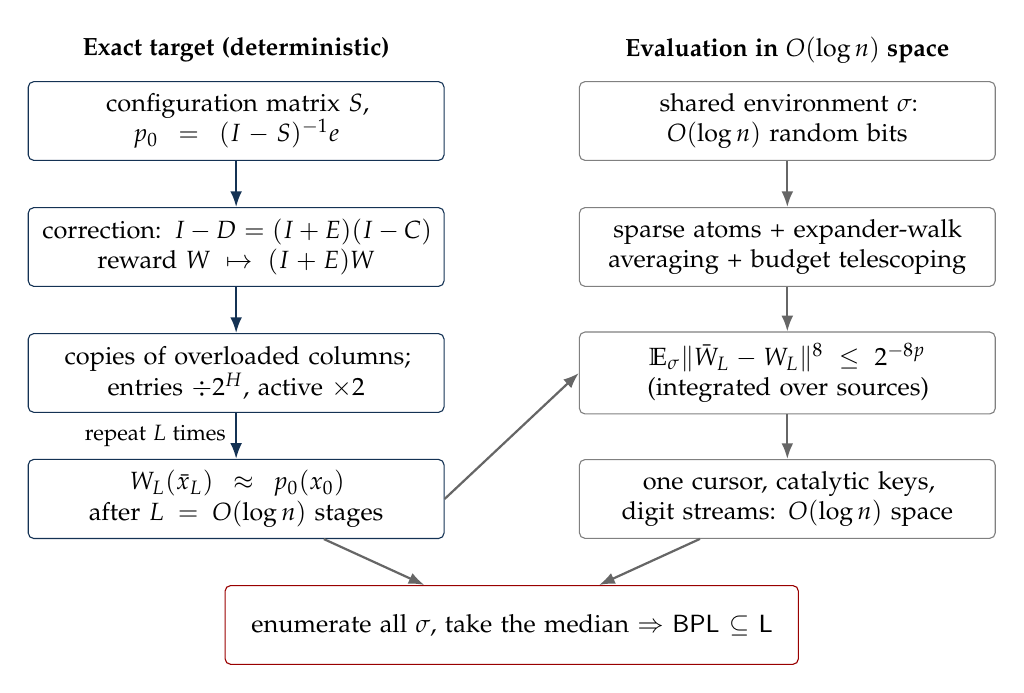
\begin{tikzpicture}[x=1cm,y=1cm,every node/.style={font=\small},
  box/.style={draw=linkblue!80!black,rounded corners=2pt,align=center,inner sep=4pt,text width=5.0cm,minimum height=10mm},
  sbox/.style={draw=black!50,rounded corners=2pt,align=center,inner sep=4pt,text width=5.0cm,minimum height=10mm},
  arr/.style={-{Latex[length=2mm]},thick,draw=linkblue!80!black},
  dsh/.style={-{Latex[length=2mm]},thick,draw=black!60}]
\node[font=\small\bfseries] at (0,0.9) {Exact target (deterministic)};
\node[font=\small\bfseries] at (7.0,0.9) {Evaluation in $O(\log n)$ space};
\node[box] (a) at (0,0) {configuration matrix $S$,\\ $p_0=(I-S)^{-1}e$};
\node[box] (b) at (0,-1.6) {correction: $I-D=(I+E)(I-C)$\\ reward $W\mapsto(I+E)W$};
\node[box] (c) at (0,-3.2) {copies of overloaded columns;\\ entries $\div2^H$, active $\times2$};
\node[box] (d) at (0,-4.8) {$W_L(\bar x_L)\approx p_0(x_0)$\\ after $L=O(\log n)$ stages};
\draw[arr] (a)--(b); \draw[arr] (b)--(c); \draw[arr] (c)-- node[left,font=\footnotesize]{repeat $L$ times} (d);
\node[sbox] (e) at (7.0,0) {shared environment $\sigma$:\\ $O(\log n)$ random bits};
\node[sbox] (f) at (7.0,-1.6) {sparse atoms + expander-walk\\ averaging + budget telescoping};
\node[sbox] (g) at (7.0,-3.2) {$\E_\sigma\|\bar W_L-W_L\|^8\le2^{-8p}$\\ (integrated over sources)};
\node[sbox] (h) at (7.0,-4.8) {one cursor, catalytic keys,\\ digit streams: $O(\log n)$ space};
\node[sbox,draw=red!60!black,text width=7.0cm] (i) at (3.5,-6.4) {enumerate all $\sigma$, take the median $\Rightarrow$ $\BPL\subseteq\Lc$};
\draw[dsh] (e)--(f); \draw[dsh] (f)--(g); \draw[dsh] (g)--(h);
\draw[dsh] (d.east)--(g.west);
\draw[dsh] (d)--(i); \draw[dsh] (h)--(i);
\end{tikzpicture}
\caption{Architecture. The left column is \cref{sec:hierarchy}; the right column is
\cref{sec:estimator,sec:space}.}
\label{fig:arch}
\end{figure}

\subsection{Status}

The manuscript is 108 pages. Its first half is the hierarchy and the statistical
estimator; its second half is the implementation (numerical streams and the
controller), the conclusion and the compiler. The repository's index lists no
Lean formalization for this result, so, unlike the Unique Games proof in the same
release, it rests on the written argument alone. The README notes that
unformalized results ``could have issues.'' Given the claim, this paper deserves
an expert referee; \cref{sec:reader} suggests where to start.

\section{The exact target: the correction and copy hierarchy}\label{sec:hierarchy}

\subsection{Acceptance probability as a matrix inverse}\label{sec:config}

\begin{lemma}[Configuration reduction; Lemma~2.1 of \cite{OpenAI-BPL}]\label{lem:config}
For a polynomial-time randomized log-space machine and input $x$ one can
specify in log space a polynomial-size vertex set $V_0$ (time-stamped
configurations), a strictly forward substochastic matrix $S$ (every nonzero entry
goes from time $t$ to time $t+1$; rows sum to at most $1$) with constant in- and
out-degree and paired ports, an indicator $e$ of accepting configurations at the
final time, and a start $x_0$, such that $p_0=(I-S)^{-1}e=\sum_jS^je$ lies in
$[0,1]^{V_0}$ and $p_0(x_0)$ is the acceptance probability.
\end{lemma}

Bounded in-degree (predecessors are found by guessing a constant amount of local
change) and \emph{paired ports} (from a vertex and an out-port one can compute the
neighbor and the corresponding in-port, and conversely) will matter later: they
let the algorithm move a single cursor along an edge and back without storing the
old address.

\subsection{Moving mass into the reward}\label{sec:correction}

The whole hierarchy rests on one identity. For square matrices $C$ and $E$,
\[
D:=C-E+EC\qquad\Longrightarrow\qquad I-D=(I+E)(I-C).
\]
So if $(I-C)p=W$, then $(I-D)p=(I+E)W$: the same vector $p$ solves the new system
with transitions $D$ and reward $W+EW$.

\begin{idea}[Reading the identity as path shortcutting.]
Think of $E(x,y)$ as the part of the transition $x\to y$ that we decide to
``pay out now''. The new reward at $x$ gains $E(x,y)W(y)$, the reward collected
at $y$; and the new transitions gain $E(x,y)C(y,\cdot)$, which continue directly
from $y$'s successors. Removing $E$ from $C$ and adding $EC$ is exactly replacing
the edge $x\to y$ by ``collect $y$'s reward and jump past $y$''. Nothing is
approximated; the identity is exact for every $E$.
\end{idea}

The point of a stage is to choose $E$ so that $D$ has \emph{small entries}. Fix a
stage with vertex set $V$, a rate $f=2^{-Hl}$, and an input $C$ that is strictly
forward, substochastic, and has entries at most $f$. Write $q=2^H$ ($H\ge4$ fixed).
A large entry of $C$ can be removed only if $E$ absorbs most of it, but $E$ also
creates new entries $EC$; those can again be large. The manuscript solves the
self-consistent equation
\[
E_*(x,y)=f\,Q\bigl((C+E_*C)(x,y)/f\bigr)\,g(y),
\]
where $Q$ is a smooth cutoff with $(t-\theta_2)_+\le Q(t)\le(t-\theta_1)_+$ for small
fixed $0<\theta_1<\theta_2<1/(32q)$, and $g\colon V\to[0,1]$ is a column multiplier
(which columns are allowed to be corrected). With $g\equiv1$, the residual
$T=C-E_*+E_*C$ has every entry at most $\theta_2f$.

\begin{lemma}[Factorial truncation; Lemma~4.1 of \cite{OpenAI-BPL}]\label{lem:factorial}
The fixed point $E_*$ exists and is unique (define each row in increasing column
order). The iterates $E_0=0$, $E_i=fQ((C+E_{i-1}C)/f)\,g$ increase to $E_*$, and
\[
\max_{x,y}\frac{E_*(x,y)-E_k(x,y)}f\le e^{1/\theta_1}\frac{(L_Q/\theta_1)^k}{k!}.
\]
So a fixed number $k_*$ of iterations, independent of $\abs V$, gets within
$f/(32q)$ of the fixed point.
\end{lemma}

\begin{proof}[Why]
The residual has rows summing to at most $1$ and every positive entry of $E_*$
leaves a residual of at least $\theta_1f$, so row $x$ of $E_*$ has at most
$m_x\le1/(\theta_1f)$ nonzero entries. Unrolling $E_*\le C+E_*C$ along row $x$
writes $E_*(x,y)$ as a sum over increasing chains $x<z_1<\dots<z_j<y$ inside
that support set, each a product of $j+1$ entries of size $\le f$. There are
$\binom{m_x}{j}$ chains, so $E_*(x,y)\le f(1+f)^{m_x}\le fe^{1/\theta_1}$. The
same unrolling for $E_*-E_k$ uses only chains of length exactly $k$, giving
$\binom{m_x}{k}f^k\le(1/\theta_1)^k/k!$.
\end{proof}

\subsection{Overloaded columns and detectors}\label{sec:detectors}

Correction is not allowed everywhere. If many rows have large entries into the
same column $y$, correcting all of them would later require handling all those
incoming entries at $y$, and the estimator needs bounded incoming degree. So the
multiplier $g(y)$ is turned off at \emph{overloaded} columns, and these are found
by a detector.

\paragraph{Sampling channels.} Vertices have numerical IDs of $O(\log n)$ bits. A
\emph{rank channel} is a random $H\times h_0$ matrix $A=(a_0,F)$ over a prime field
$\F_P$, $P=2^{\Theta(\log n)}$, with $F$ of full column rank. A vertex $y$ is
\emph{retained at rate $b_k=2^{-Hk}$} if all $H$ coordinates of
$A(1,y,\dots,y^{h_0-1})^\top$ lie in $\{0,\dots,\lceil P2^{-k}\rceil-1\}$. This is a
pairwise-independent-style sample with
\[
\Pr[\text{retained}]=\pi_{b}\asymp b,\qquad
\Pr[y\text{ retained}\mid x\text{ retained}]\le C\,b\ (x\ne y),
\]
and Chebyshev tails for counts (Lemma~3.1 of \cite{OpenAI-BPL}). Channels $X$
(sources), $Y$ (terminals) and a few more are independent. The whole collection,
plus some auxiliary bits, is the \emph{environment} $\sigma$; it has $O(\log n)$
bits.

\paragraph{The detector.} At pilot step $i$ let $G_i=C+\widehat E_{i-1}C$. A row
gate $R_i(x)$ is $1$ when row $x$ has fewer than $K$ retained large entries. The
column score
\[
U_i(y)=\E\Bigl[\operatorname{rank}_J\{\phi(G_i(x,y)/f)R_i(x):X_f(x)=1\}\ \Big|\ Y_f(y)=1\Bigr]
\]
is a \emph{deterministic} number: an expectation over the channels of the $J$-th
largest score among sampled rows. Set
$\widehat g_i(y)=\gamma(\max_{r\le i}U_r(y))$, where the cutoff $\gamma$ is $1$ for
scores up to $1/2$ and $0$ from $4/5$ on, and after $k_*$ pilot steps use $g=\widehat g_{k_*}$ in the
actual iteration.

\begin{lemma}[Detectors; Lemma~4.3 of \cite{OpenAI-BPL}]\label{lem:detector}
If more than $R_*/f$ rows have $G_i(x,y)\ge\delta_1f$, then $U_i(y)\ge19/20$.
If $U_i(y)>1/4$, then more than $J/(4C_\pi f)$ rows have $G_i(x,y)>\delta_0f$.
Hence a corrected column ($g(y)>0$) has at most $R_*/f$ large incoming entries.
\end{lemma}

The first statement is sampling: about $R_*\pi_f/f\gg J$ heavy rows are retained,
and most have full row gates. The second is Markov's inequality. Thresholds are
smooth cutoffs so that everything is later Lipschitz in its inputs.

\begin{lemma}[Residual; Lemma~4.4 of \cite{OpenAI-BPL}]\label{lem:residual}
With $E=E_{k_*}$ and $D=C-E+EC$: $D$ is nonnegative, strictly forward and
substochastic; $D(x,y)\le(k_*+1)f$; and $D(x,y)\le\eps_{\rm good}f<f/(16q)$ in
every column with $g(y)=1$. Moreover $D\ge c\,(C+E+EC)$ for a fixed $c>0$.
\end{lemma}

The last inequality says the three unsigned terms of $D$ are each dominated by
$D$, so later each can be estimated separately with error measured relative to $D$.

\subsection{Copies}\label{sec:copies}

Entries of $D$ are now small in good columns but can still be about $f$ in
overloaded ones. Make $D_0>K_*q$ copies $y_0,\dots,y_{D_0-1}$ of every vertex, and
route large entries evenly:
\[
C^+(x_i,y_j)=r_i(x)\,D(x,y)\,s_j(D(x,y)/f),
\]
where $s_0\approx1$ and $s_j\approx0$ for small entries, $s_j=1/D_0$ for all $j$ when
the entry exceeds $f/(4q)$, and the row factor $r_j(x)$ ($j>0$) is $1$ only for
vertices whose detector score was high. Let $P^r(x_i,x)=r_i(x)$.

\begin{proposition}[One stage; Prop.~4.5 of \cite{OpenAI-BPL}]\label{prop:stage}
$C^+$ is strictly forward and substochastic, $C^+\le f/q$ entrywise,
$C^+P^r=P^rD$, and $\abs{\mathcal A(C^+)}\le2\abs{\mathcal A(C)}$, where
$\mathcal A$ is the set of vertices touching a positive entry.
\end{proposition}

\begin{proof}[Why]
Entries: a small entry stays below $f/(4q)$; a large one is split $D_0$ ways and
is at most $K_*f/D_0<f/q$. Intertwining: on any positive entry the routing
fractions times row factors sum to $1$, because a large entry in a column forces
that column to be uncorrected, hence high-scoring, hence $r_j=1$. Active count:
only high-scoring parents $\mathcal O$ get extra active copies. Each has more than
$J/(4C_\pi f)$ incoming entries above $\delta_0f$, while the total number of such
entries is at most $\abs{\mathcal A(C)}k_*(k_*+1)/(2\delta_0f)$ (row sums are at
most $k_*$). With $J$ large, $(D_0-1)\abs{\mathcal O}\le\abs{\mathcal A(C)}$.
\end{proof}

\subsection{The target}\label{sec:target}

Start from $C_0=S$, $W_0=e$, and iterate with $f_l=q^{-l}$,
$V_{l+1}=V_l\times\{0,\dots,D_0-1\}$, $C_{l+1}=C_l^+$, and
\[
W_{l+1}(x_i)=r_i(x)\bigl(W_l(x)+(E_lW_l)(x)\bigr).
\]

\begin{proposition}[Prop.~4.7 of \cite{OpenAI-BPL}]\label{prop:target}
With $P_l^c$ the cumulative projection, $W_l=P_l^cp_0-C_lP_l^cp_0$ and $0\le W_l\le1$.
For the all-primary copy $\bar x_l$ of a base vertex $x$,
\[
0\le p_0(x)-W_l(\bar x_l)\le\abs{V_0}\,2^{-(H-1)l}.
\]
Hence $L=O(\log n)$ stages give any fixed inverse-polynomial accuracy, and every
$V_l$ has $2^{O(\log n)}$ vertices with $O(\log n)$-bit addresses.
\end{proposition}

\begin{proof}
By induction $C_lP_l^c=P_l^c-B_l(I-S)$ with $B_{l+1}=P^r_l(I+E_l)B_l$, using
$C^+P^r=P^rD$ and $I-D=(I+E)(I-C)$. Apply this to $p_0$ and use $(I-S)p_0=e$. Every
row of $C_l$ has at most $2^l\abs{V_0}$ positive entries, each at most $q^{-l}$, so
its sum is at most $\abs{V_0}2^{-(H-1)l}$, and $0\le P_l^cp_0\le1$ with
$(P_l^cp_0)(\bar x_l)=p_0(x)$.
\end{proof}

\begin{idea}[What the hierarchy buys.]
Every stage is exact, and the number of stages is $O(\log n)$. The probability
does not have to be computed by multiplying out long paths; it has been
``pushed'' into a reward vector by a logarithmic number of local, sparse
corrections. The price is that each stage is defined through the previous one,
through nonlinear cutoffs, and through expectations over hash functions. The
rest of the paper is about evaluating this object without $O(\log n)$ bits per
stage.
\end{idea}

\section{Estimating the target with a shared random environment}\label{sec:estimator}

This section and the next describe how $W_L(\bar x_L)$ is evaluated. Here the
question is statistical: what is computed, and why is it accurate for most
environments? \Cref{sec:space} explains why each computation fits in $O(\log n)$
space. Proofs in the manuscript are long; this section aims to make the
statements and their purposes clear, with the main estimates indicated.

\subsection{What has to be estimated}\label{sec:env}

At each stage the hierarchy uses a fixed list of \emph{tasks}, in a fixed
dependency order: entries of $C_l$; at each pilot step the detector scores and the
vector $U_i$; the pilot and actual corrections $E_i$; entries of $D_l$ routed to
copies; and the reward update $W_{l+1}$. A \emph{row task} is a whole sparse table
(an estimate of one of these matrices); a \emph{vector task} is a vertex function.
The number of task types per stage is a constant, so there are $O(L)=O(\log n)$
task ranks in all.

All tasks share one random \emph{environment} $\sigma$: a constant number of
independent rank channels (\cref{sec:detectors}) over a field of size
$P=2^{\Theta(\log n)}$, plus $O(\log n)$ auxiliary ``salt'' bits used for
fingerprints (\cref{sec:fingerprints}). The environment is shared by every task at
every level. No independence between the errors of different tasks is ever
assumed; all bounds are proved by triangle inequalities, H\"older, and caps on
degrees.

\subsection{Atoms: sparse tables with exact conditional means}\label{sec:atoms}

A matrix entry $G(x,y)$ at stage rate $f$ is represented on the slice where the
source is retained at rate $u$ and the terminal at rate $a$ (written
$X_u(x)=Y_a(y)=1$). Entry sizes are split into scale bins
$G=\sum_kG\,\omega_k(G)$, with $\omega_k$ a smooth partition of unity on dyadic
scales $b_k=2^{-Hk}$. At scale $a$ the \emph{dense atom} is
\[
\mathcal B_a(x,y)=\one_{\{Y_t(y)=1\}}\frac{k_a(G(x,y)/a)\,R(x)}{c(q_y)},
\]
where $k_a$ is the bin function, $R(x)\in[0,1]$ is a row gate that vanishes when
row $x$ has $K$ or more retained large entries, and $q_y$ is the exact conditional
mean of the gate (a ``preparatory'' table), clipped to $[1/2,1]$.

\begin{lemma}[Atom identities; Lemmas~5.1 and 5.3 of \cite{OpenAI-BPL}]
On the slice $X_u(x)=Y_t(y)=1$, the conditional mean of $a\,\mathcal B_a(x,y)$ is
exactly $G(x,y)\omega_k(G(x,y))$. Each row of an atom table has fewer than $K$
nonzero entries. Correction atoms carry an additional incoming gate, so each
column of an exposed correction relation has at most $K_c$ entries; their
conditional means are exactly the corrections.
\end{lemma}

Products are estimated by sampling midpoints: an entry of $EC$ is represented by
$\frac{f}{\pi_f}\sum_{z:Z_f(z)=1}\mathcal F(x,z)\mathcal B_b(z,y)$, which has the
right conditional mean because the channels $X$, $Z$, $Y$ are independent and the
true atoms factor through them (Lemma~7.1 of \cite{OpenAI-BPL}).

\begin{idea}[Why sparse tables, and why exact means.]
Bounded row and column support is what lets a single cursor walk along table
entries (\cref{sec:space}). Exact conditional means are what make the
estimator's errors telescope in \cref{sec:budget}: the target of every sample
term is a deterministic number, so the error can be split into a deterministic
bias and a mean-zero noise, which are bounded by different arguments.
\end{idea}

\paragraph{The error metric.} For a row quantity $Z$ and $s=8$,
\[
\|Z\|_{u,a;s}^s=\frac1N\,\E_\sigma\sum_x\frac{X_u(x)}u\sum_{y:Y_a(y)=1}\abs{Z(x,y)}^s,
\qquad N=2^{C_N\log n}\ \text{(a bound on stage size)},
\]
and errors of bounded nonnegative outputs are measured in the root discrepancy
$\|H^{1/s}-(H')^{1/s}\|$. Three features matter: the error is \emph{averaged over
sources} (weight $X_u/u$, normalized by $1/N$); it is an $L^8$ norm over the
environment; and taking $8$th roots turns multiplicative errors into additive
ones. At the very end, passing from an average over sources to one specific start
costs a factor $N=n^{O(1)}$ (\cref{sec:finish}), which is paid by making the
statistical precision a large constant times $\log n$.

\paragraph{The cost of releasing a source.} In a product
$\mathcal F(x,z)\mathcal B_b(z,y)$ the right factor's error is measured with
sources $z$ at rate $f$, not $x$ at rate $u\le f$. Because correction atoms have at
most $K_c$ incoming entries, each $z$ is reached from at most $K_c$ sources, and the
change of source domain costs a factor $f/u$ in the $s$-th power of the norm
(Lemma~7.3 of \cite{OpenAI-BPL}). This is paid by the precision convention below.

\subsection{Conditional averaging with property (T)}\label{sec:averaging}

Every atom identity is a conditional mean on a slice of environments. To
approximate such a mean for a function $F(\sigma)$, the estimator replaces
$F(\sigma)$ by the average of $F$ over the endpoints of all walks of length $d$ from
$\sigma$ (a deterministic sum over $2^{O(d)}$ walk words). If the walk has a
spectral gap on the slice, this is close to the conditional mean.

\begin{lemma}[Uniform gap; Lemmas~6.1--6.2 of \cite{OpenAI-BPL}]
Let $G_H=\mathrm{SL}_H(\mathbb Z)\ltimes\mathbb Z^H$ with $H\ge3$ and a fixed
finite symmetric generating set. The lazy walk has a spectral gap, depending only
on $H$, on every finite transitive $G_H$-set. Consequently there is a Markov
operator $K$ on each conditional slice of environments with
$\|K^d-\Pi\|_{L_s\to L_s}\le C_s2^{-c_sd}$, uniformly in the field size, the box
sizes, and the conditioning vertices.
\end{lemma}

The action is on a channel's coordinates $(F,w)$, where $F$ is the frame and
$w=A(1,y,\dots,y^{h_0-1})^\top$ is the retained box coordinate of the conditioning
vertex $y$: $(M,c)$ acts by $(F,w)\mapsto(MF,Mw+c)$. It is transitive, so the gap
follows from property~(T) of $\mathrm{SL}_H(\mathbb Z)$ and relative property~(T) of
$(\mathrm{SL}_2(\mathbb Z)\ltimes\mathbb Z^2,\mathbb Z^2)$, with Shalom's explicit
Kazhdan constants~\cite{Shalom}; Riesz--Thorin moves the $L_2$ gap to $L_8$.

\begin{idea}[Why property (T) instead of an ordinary expander.]
The algorithm must average over environments conditioned on retaining vertices
it does not currently remember. So each walk step must be a fixed,
measure-preserving transformation of the environment that does not mention the
conditioning vertex, with validity checked only when the vertex is visited
(Lemma~6.3: ``guessed wraps'' are enumerated and exactly one survives). A group
action does this naturally, and property~(T) gives one spectral gap for all the
finite quotients that arise, whatever the field size and box sizes.
\end{idea}

\subsection{The budget schedule}\label{sec:budget}

Each task has an integer \emph{statistical budget} $M$ and an implicit precision
\[
p=\frac{M}{K_{\rm prec}}-\frac12\log_2\frac1a-\frac12\log_2\frac1u-A_*\,i_*,
\]
where $a,u$ are its end and start rates and $i_*$ its rank in the dependency
order. Tasks with $p\le0$ return zero. The inductive claim is that every task's
error is at most $C_b2^{-p}$. The $\frac12\log$ terms are exactly what pays for
scale changes (a bin at scale $b$ costs $(b/a)^{1/8}$ or $(b/a)^{7/8}$, and weight
$1/2$ sits between these) and for releasing a source (cost $(f/u)^{1/8}$).

\paragraph{Additive estimation.} A task at budget $M$ is computed as
\[
\text{exact base terms}\;+\sum_{b}\ \sum_{m=1}^{M-c_b}K^{\ell(M-m)}\bigl(T_{b,m}-T_{b,m-1}\bigr),
\]
where $T_{b,m}$ is a sample term using child estimates at budget $m$, $c_b\approx
c_0(1+\abs{\log_2(b/a)})$ cuts off scales far from $a$, and $K^{\ell(M-m)}$ is the
conditional walk of length proportional to the slack $M-m$. The conditional means
telescope to the term at the largest available budget, whose bias is bounded by
induction (Lemma~7.6). The noise of each difference is small because both terms
approximate the same quantity (Lemma~7.7 gives $2^{-p+C_0(M-m)}$ before
averaging), and the walk contracts it by $2^{-c\ell(M-m)}$, which wins for a
large fixed $\ell$ (Lemma~7.8).

\begin{idea}[A multilevel estimator.]
This is in the spirit of multilevel Monte Carlo: accurate children are used
sparingly and with little averaging, cheap children often and with much
averaging. Its real purpose here is space. A term at slack $d=M-m$ is described
by $O(d)$ bits (walk word, scale offset, formula choices; Lemma~7.5), and calls a
child of budget at most $M-d$. That is the exchange rate the space accounting
of \cref{sec:space} needs.
\end{idea}

\subsection{Compression of rows}\label{sec:compression}

Adding many increments can make a row array dense. After each dyadic slack group
$d_j$, the array is replaced by a common default plus a list of at most
$n_j=2^{c_2d_j}$ exceptions: the threshold is the largest of the old default, a
floor $\rho_j=2^{-c_1d_j}$, and the $n_j$-th largest entry size; everything below
twice the threshold becomes the default (Lemma~8.1). The map is uniformly Lipschitz.

The analysis (Section~8) separates three cases. Before the first ``overflow''
(threshold above the floor), all changes are tiny. An overflow caused by genuinely
many heavy endpoints is rare: total row mass is bounded, so the expected number of
retained heavy endpoints, even conditioned on one endpoint, is $O(1/\rho_j)$, and
Markov gives probability $O(1/(n_j\rho_j))$. An overflow caused by errors at light
endpoints is charged to those errors. With $c_2$ large relative to $c_1$, all the
resulting series converge (Prop.~8.5), so compression costs only a constant
factor in the error. Range clamps (Lemma~8.6) keep numbers in $O(d)$ bits without
changing any relevant output.

\subsection{Fingerprints within budget blocks}\label{sec:fingerprints}

Comparing two endpoint IDs exactly needs $O(\log n)$ bits, but a frame at small
slack $d$ may keep only $O(d)$ bits. For slack $d\le2h_*$, where
$h_*=\lfloor\eps\log_2B\rfloor=\Theta(\eps\log\log n)$, endpoints are therefore compared by keys
$k(v)\in\{1,\dots,B\}$: $k(v)=\tau(\alpha P_v(r)+\beta)$ over a prime near $B^3$,
with $P_v$ the polynomial whose coefficients are the bits of $v$. Distinct fixed
IDs collide with probability $O(1/B)$ (Lemma~9.1).

The difficulty is \emph{adaptivity}: which endpoints get compared depends on
earlier computations, which may depend on the key. The manuscript handles this as
follows (Section~9).
\begin{itemize}
\item Budgets are cut into blocks of $h_*$ consecutive values, each with an
  independent salt. A task in block $b$ may look only at salts of blocks $\le b$;
  its walks vary the earlier salts and freeze the rest.
\item A \emph{clean calculation} uses exact ID comparison inside the current
  block. It is independent of the block's salt (Lemma~9.2).
\item The clean calculation determines an \emph{envelope} of at most $2^{O(h_*)}$
  candidate endpoints per row, independent of the salt, so all keys in it are
  distinct except with probability $2^{O(h_*)}B^{-1/2}$ (Lemma~9.3).
\item Actual candidates outside the envelope are charged to child errors, using
  smooth ``witness'' functions (Lemma~9.4); collisions inside it are charged
  directly (Lemma~9.6); bucket sums only alias increments, never stored values
  (Lemma~9.5).
\item A coupled induction bounds the actual--clean discrepancy by
  $2^{-p}2^{-D_1h_*+D_2(M-M_b)}$, closed by choosing $\eps$ small (Prop.~9.7).
\end{itemize}

\begin{theorem}[Estimator accuracy; Theorem~9.8 of \cite{OpenAI-BPL}]\label{thm:estimator}
Every task output satisfies the error bound $C_b2^{-p}$. In particular,
\[
\frac1N\E_\sigma\sum_{x\in V_l}\frac{X_u(x)}u\abs{\bar W_l(x)-W_l(x)}^8\le C_b^8\,2^{-8p},
\]
with constants independent of the input and of $\log n$.
\end{theorem}

\section{Fitting the estimator into logarithmic space}\label{sec:space}

Fix an environment $\sigma$. Every estimator value is now a deterministic finite
recursion. The manuscript's Sections~10--11 show that a single deterministic
machine evaluates any requested binary digit of any task value in $O(\log n)$
space, on \emph{every} environment, including the ones where the estimate is
inaccurate. Totality matters: the final enumeration must finish on every
environment.

\subsection{What is kept, and what is shared}

The shared facilities, present once for the whole computation, are: the input;
the master environment ($O(\log n)$ bits); a single \emph{cursor} holding one
vertex ID; a \emph{catalytic} bit vector of length $B$; and one scratch area of
$O(\log n)$ bits whose contents never survive a recursive call. Everything else
is a suspended \emph{local record} of a caller waiting for a lower query. The
whole difficulty is to bound the sum of local records along the active call chain.

\paragraph{One cursor and paired ports.} A product term
$\mathcal F(x,z)\mathcal B(z,y)$ is evaluated with the cursor at $x$: a correction
port moves it to $z$ and returns a bounded inverse port, the right factor is
queried at $z$ with a task description that does not mention $x$, and the
inverse port moves the cursor back. No second vertex address is ever stored
across a recursive call (Theorem~11.1).

\paragraph{Incoming edges by tree contours.} Some operations need the incoming
entries of a column (the incoming gate of corrections, incoming ranks). These
are found by viewing the deterministic program that maps a row port to its
endpoint as a graph on program states. The component of a given success state is
a tree directed toward it, whose leaves of the right kind are exactly the ports
ending there. The Cook--McKenzie rotation/edge-flip contour~\cite{CookMcKenzie}
enumerates them without storing an address, as in reversible simulation of
space-bounded computation~\cite{LMT} (Lemmas~11.5--11.7).

\paragraph{Catalytic key equality.} At small slack, two endpoints are compared
by their keys, but even a $\log B$-bit key cannot be kept in every frame. The
shared vector $V\in\{0,1\}^B$ is used instead: visit $v$ and flip $V_{k(v)}$; visit
$w$ and xor $V_{k(w)}$ into a result bit; visit $v$ and flip $V_{k(v)}$ back; visit $w$
and xor $V_{k(w)}$ into the result again. The result changes by exactly
$\one[k(v)=k(w)]$ and $V$ is restored, whatever its contents were. Only a phase
and one bit are kept locally (Lemma~9.9). This is the transparent-program trick
of catalytic computing~\cite{BCKLS}.

\paragraph{Digit-by-digit arithmetic.} Values are never stored in full. A query
asks for one digit, in a redundant signed-digit stream with digits in
$\{-6,\dots,6\}$, obtained from integers $N_t$ with $\abs{N_t-2^tz}<2$ by
$z_t=N_t-2N_{t-1}$ (Lemma~10.1). Products, reciprocals (for the normalizations
$1/c(q_y)$), ranks and sums are computed by circuits evaluated depth-first from
regenerated gate addresses. A query for digit $t$ that requests an operand digit
$j$ keeps at most $ad+b(t-j)$ local bits, with $j\le t+cd$ (Theorem~10.9). So the
numerical ``clock'' also telescopes.

\subsection{The potential argument}

Give every operation an \emph{allowance}
\[
w=K_1(1+M)-(K_0+s_0)\,d,
\]
where $M$ is its budget, $d$ its slack and $s_0$ its position among a bounded
number of operation strata. Every permitted descent (to a later stratum, to a
coarser slack group, or to a child of budget at most $M-d$) lowers $w$ by at least
a constant times $d$. Combined with the numerical clock $t$, the potential
\[
\Phi(w,t)=Aw+Dt
\]
pays for each suspended segment: a frame waiting at $(w_i,t_i)$ for a query at
$(w_{i+1},t_{i+1})$ keeps at most $\Phi(w_i,t_i)-\Phi(w_{i+1},t_{i+1})$ bits. Summing
along the chain telescopes to $\Phi(w_{\rm top},t_{\rm top})=O(M_{\rm top}+t_{\rm top})=O(\log n)$.
A second potential $\Psi=t+a'w$ never increases, which bounds every clock and
therefore every scratch computation by $O(\log n)$ (proof of Theorem~11.1).

\begin{idea}[Why this beats $\log^{3/2}n$.]
In Savitch-style or Saks--Zhou-style recursion, every level of the recursion keeps
a full vertex address or a full random seed. Here a level at slack $d$ keeps
$O(d)$ bits, and the levels' slacks add up to the top budget. The cursor carries
the only vertex address; the catalytic vector carries the only key table; the
environment carries all the randomness, once. Each of these devices removes one
of the $\Theta(\log n)$-per-level costs.
\end{idea}

\begin{theorem}[Realization; Theorem~11.1 of \cite{OpenAI-BPL}]\label{thm:realize}
For every environment and every reachable task, every bit test and every digit
query terminates, returns its defined value, restores the cursor and the
catalytic vector, and uses $O(\log n)$ total space when the top budget and the
requested clock are $O(\log n)$.
\end{theorem}

\section{Finishing the proof}\label{sec:finish}

\subsection{From an average to one start, and the median}

\begin{lemma}[One start; Lemma~12.2 of \cite{OpenAI-BPL}]\label{lem:onestart}
If $\frac1N\E\sum_v\frac{X_f(v)}f\abs{\bar W(v)-W(v)}^8\le C_b^82^{-8p}$, then for any fixed $z$,
\[
\Pr\bigl[\abs{\bar W(z)-W(z)}>\eta\mid X_f(z)=1\bigr]\le N\frac f{\pi_f}C_b^82^{-8p}\eta^{-8}.
\]
\end{lemma}

\begin{proof}
Keep only the summand $v=z$ and apply Markov's inequality.
\end{proof}

\begin{proof}[Proof of \cref{thm:approx} for fixed $d$ (Theorem~12.1 of \cite{OpenAI-BPL})]
Let $r=d\lceil\log_2(n+2)\rceil$ and $\Delta=2^{-r}$. Choose $L=O(\log n)$ so that
$0\le p_{\mathcal M}(x)-W_L(z)\le\Delta/8$ for the all-primary copy $z$ of the start
(\cref{prop:target}). Choose the top budget $M_{\rm top}=O(\log n)$ so large that
$8p\ge8r+C_N\log n+O(1)$. Then \cref{lem:onestart} with $\eta=\Delta/8$ shows that
$\abs{\bar W_L(z)-W_L(z)}\le\Delta/8$ for at least $7/8$ of the environments that
retain $z$.

Enumerate all environment encodings (field matrices with a full-rank frame, and
raw salt strings) that retain $z$; there are $2^{O(\log n)}$, each of $O(\log n)$ bits.
For each, compute $K=r+6$ signed digits of $\bar W_L(z)$ (\cref{thm:realize}),
form the dyadic number $v_\sigma$, and clip it to $[0,1]$; the truncation error is
below $\Delta/8$. More than $3/4$ of the $v_\sigma$ lie within $3\Delta/8$ of
$p_{\mathcal M}(x)$, so their median does too. Find the median by binary search over
$[0,2^K]$, recounting with a fresh pass each time; only counters and the current
environment are stored. Each digit query is a halting $O(\log n)$-space
computation, hence takes $2^{O(\log n)}$ steps, and there are $2^{O(\log n)}$
queries, so the time is polynomial.
\end{proof}

\begin{proof}[Proof of \cref{thm:main}]
Apply the theorem with $d=3$ to a $\BPL$ machine: the output is within $1/8$ of the
acceptance probability, so comparing it with $1/2$ decides the language in
$\Lc$. Trivially $\Lc\subseteq\RL\subseteq\BPL$.
\end{proof}

\subsection{Consequences}\label{sec:consequences}

\begin{itemize}
\item \textbf{Promise problems.} The same algorithm is total, so
  $\mathsf{PromiseBPL}=\mathsf{PromiseL}$ (Cor.~12.3).
\item \textbf{Accuracy as input.} Padding the input to length about $n2^q$
  and running the fixed-accuracy algorithm on a virtual padded string gives error
  $2^{-q}$ in space $O(\log n+q)$ and time $n^{O(1)}2^{O(q)}$.
\item \textbf{Finding accepting runs.} If $p_{\mathcal M}(x)\ge n^{-c}$, a
  deterministic log-space transducer outputs an accepting computation: estimate
  the continuation probability of every successor configuration to accuracy
  $n^{-c}/(8T(n))$ and follow a maximum (Cor.~12.4). The error per step is
  additive and deterministic, so no simultaneous-success event is needed.
\item \textbf{An effective compiler.} One fixed randomized interpreter with
  enforced resource caps, together with the separator for it, yields an algorithm
  that, given a randomized machine and claimed bounds $(n+2)^a$ time and
  $b\log n$ space, outputs a deterministic machine with explicit bounds
  $K\log n$ space and $H(n+2)^c$ time (Theorem~13.1).
\end{itemize}

\subsection{The order of constants}

As with every proof of this kind, correctness depends on choosing constants in
the right order (Section~12.1 of the manuscript):
\begin{enumerate}
\item channel shape $H,h_0$ and the moment $s=8$ (the walk gap is uniform in all later sizes);
\item correction thresholds, the cutoff $Q$, and the iteration count $k_*$;
\item copy count $D_0$, routing and gate thresholds, row-gate rank $K$;
\item detector rank $J$, overload bound $R_*$, incoming rank $K_c$;
\item precision coefficients, compression floors and capacities, walk length;
\item crude propagation constants, then block constants $D_2,D_1$ and the block width $\eps$;
\item controller allowance and guard constants;
\item the top-budget coefficient, the field-size exponent, and the minimum size of $B$.
\end{enumerate}

\section{A guide for the careful reader}\label{sec:reader}

\subsection{What this note does and does not establish}

This note describes the manuscript's proof; it is not a verification. I checked
the algebra of the hierarchy in \cref{sec:hierarchy} (the transfer identity, the
reward identity, the row-sum bound, the factorial truncation argument, the
active-vertex count) and the final enumeration and median argument, and found
them correct. For \cref{sec:estimator,sec:space} I read the manuscript's
statements and arguments and have tried to report them faithfully, but those
sections are long and intricate, and I did not check them line by line. There is
no Lean formalization of this result in the repository.

\subsection{Where to look hardest}

\begin{enumerate}
\item \textbf{The hierarchy} (Section~4). It is elementary and the cleanest part.
  Its role is to reduce the problem to an exact object with $O(\log n)$ stages and
  bounded local structure. It is worth checking independently, since if it is
  right it is already a new structural fact about substochastic forward matrices.
\item \textbf{Shared randomness without independence} (Sections~5--7). Every
  task at every level uses the same $O(\log n)$-bit environment. The proofs claim
  never to need independence between the errors of different tasks. The places to
  test this are products (Lemma~7.3), where a left factor's support is used to
  sum a right factor's error, and the use of conditional means on slices.
\item \textbf{Conditional averaging} (Section~6). Check that the validated
  walk variants really average exactly over the conditioned slice and that each
  sample function depends only on coordinates the walk varies (the
  ``determinism hypothesis'' of Lemma~7.8 and Lemma~9.2).
\item \textbf{Compression} (Section~8). The conditional-rarity argument
  (Lemma~8.4) applies to deterministic mean errors but not to noise; the proof
  handles noise separately using uniqueness of the first overflow. This split is
  delicate.
\item \textbf{Adaptive fingerprints} (Section~9). The salt-visibility rule must
  hold for every access operation, including inverse queries and port orders, not
  only for numerical values (Lemma~11.11 implements it). An error here would
  break the independence of the envelope from the block's salt.
\item \textbf{Space accounting} (Sections~10--11). The claim is that every
  retained bit is charged to a decrease in allowance or clock. Look at the
  contour traversal of program graphs that include ``opaque'' lower queries, and
  at the guard construction for synthetic predecessor states.
\end{enumerate}

\subsection{Correspondence with the manuscript}

\begin{center}\small
\renewcommand{\arraystretch}{1.15}
\begin{tabular}{@{}ll@{}}
\toprule
\textbf{This note} & \textbf{Manuscript} \\
\midrule
\cref{thm:main,thm:approx} & Theorems 1.1, 1.2, 12.1 \\
\cref{lem:config} & Lemma 2.1 (Section 2) \\
Rank channels (\cref{sec:detectors}) & Section 3, Lemma 3.1 \\
\cref{lem:factorial,lem:detector,lem:residual} & Lemmas 4.1, 4.3, 4.4 \\
\cref{prop:stage,prop:target} & Propositions 4.5, 4.7 \\
Atoms (\cref{sec:atoms}) & Section 5 \\
Averaging (\cref{sec:averaging}) & Section 6 \\
Budget schedule (\cref{sec:budget}) & Section 7 \\
Compression (\cref{sec:compression}) & Section 8 \\
Fingerprints (\cref{sec:fingerprints}), \cref{thm:estimator} & Section 9, Theorem 9.8 \\
Digit streams & Section 10, Theorem 10.9 \\
\cref{thm:realize} & Section 11, Theorem 11.1 \\
\cref{lem:onestart}, finish, consequences & Section 12 \\
Compiler & Section 13 \\
\bottomrule
\end{tabular}
\end{center}


\begin{thebibliography}{99}\small
\bibitem{OpenAI-BPL} OpenAI. \emph{Exact Derandomization of Logarithmic Space: $\mathsf L=\mathsf{RL}=\mathsf{BPL}$.} Manuscript, September 23, 2026. \url{https://github.com/openai/math}.
\bibitem{AKLLR} R.~Aleliunas, R.~Karp, R.~Lipton, L.~Lov\'asz, C.~Rackoff. Random walks, universal traversal sequences, and the complexity of maze problems. FOCS 1979.
\bibitem{BCKLS} H.~Buhrman, R.~Cleve, M.~Kouck\'y, B.~Loff, F.~Speelman. Computing with a full memory: catalytic space. STOC 2014.
\bibitem{CarterWegman} J.~L.~Carter, M.~N.~Wegman. Universal classes of hash functions. \emph{J.\ Comput.\ Syst.\ Sci.} 18(2), 1979.
\bibitem{ChengHoza} K.~Cheng, W.~Hoza. Hitting sets give two-sided derandomization of small space. \emph{Theory of Computing} 18, 2022.
\bibitem{CookMcKenzie} S.~Cook, P.~McKenzie. Problems complete for deterministic logarithmic space. \emph{J.\ Algorithms} 8(3), 1987.
\bibitem{Hoza21} W.~Hoza. Better pseudodistributions and derandomization for space-bounded computation. RANDOM 2021.
\bibitem{LMT} K.-J.~Lange, P.~McKenzie, A.~Tapp. Reversible space equals deterministic space. \emph{J.\ Comput.\ Syst.\ Sci.} 60(2), 2000.
\bibitem{Nisan92} N.~Nisan. Pseudorandom generators for space-bounded computation. \emph{Combinatorica} 12(4), 1992.
\bibitem{Nisan94} N.~Nisan. $\mathsf{RL}\subseteq\mathsf{SC}$. \emph{Computational Complexity} 4, 1994.
\bibitem{Reingold} O.~Reingold. Undirected connectivity in log-space. \emph{J.\ ACM} 55(4), 2008.
\bibitem{SaksZhou} M.~Saks, S.~Zhou. $\mathsf{BP_HSPACE}(S)\subseteq\mathsf{DSPACE}(S^{3/2})$. \emph{J.\ Comput.\ Syst.\ Sci.} 58(2), 1999.
\bibitem{Shalom} Y.~Shalom. Bounded generation and Kazhdan's property (T). \emph{Publ.\ Math.\ IH\'ES} 90, 1999.
\end{thebibliography}
\end{document}
